
\documentclass{ssc}

% Additional packages
\usepackage[main=english,slovak]{babel}
% For thesis written in English just change the order of languages:
% \usepackage[main=english,slovak]{babel}

\usepackage{listings}  % for source code
% Listings settings
% See for details: https://en.wikibooks.org/wiki/LaTeX/Source_Code_Listings
\usepackage{qtree}
\usepackage{tikz-qtree}
\usepackage{graphicx}
\usepackage{subcaption}

\lstset{
    basicstyle=\small\ttfamily,  % smaller typewriter font
    showstringspaces=false       % don't show spaces in string
}

% Location of file with bibliography resources
\addbibresource{bibliography.bib}


%Variables
%\thesisspec{figures/thesisspec.png} 

\title{Automatic prediction model builder}{Automatická tvorba predikčných modelov}

\author[Bc.]{Aleš}{Jandera}
\supervisor{doc. Ing. Tomáš Škovránek, PhD.} %veduci prace
%\college{University of Žilina}{Žilinská univerzita} %univerzita
%\faculty{Faculty of Electrical Engineering and informatics}{Fakulta elektrotechniky a informatiky} %fakulta
%\department{Department of Computers and Informatics}{Katedra počítačov a informatiky} %katedra
%\departmentacr{DCI}{KPI} % skratka katedry
\submissiondate{21}{4}{2023}
%\fieldofstudy{Process control of raw materials and material extraction and processing}
%\studyprogramme{Cybernetics}
%\city{Košice} %mesto
\keywords{Mathematic modeling, forecasting, linear prediction, neural netowrk, prediction model builder}{Matematické modelovanie, predpoved, lineárna predikcia, neurónová sieť}

\abstract{%
    % english 
	Neural network data classification has been successfully applied to a wide
    range of data classification problems. This paper presents a Neural Network Data
    Classification model builder system in the form of an application with a user-friendly
    user interface. The application is based on a combination of machine learning
    algorithms with a statistical approaches such as Monte Carlo and Markov chains.
    The classification of the data is carried out using a machine learning algorithm,
    which provides the optimal solution for the creation of the prediction model.
    Application is created in Matlab.
}{%
    % slovak 
	Klasifikácia údajov neurónovej siete bola úspešne aplikovaná na širokú škálu
    problémov klasifikácie údajov. Táto práca predstavuje systém na tvorbu predikčých
    modelov vo forme aplikácie s užívateľsky prívetivým užívateľským rozhraním.
    Aplikácia je založená na kombinácii algoritmov strojového učenia so statistickými
    metódami ako sú Monte Carlo a Markovove reťazce. Klasifikácia údajov sa vykonáva
    pomocou algoritmu strojového učenia, ktorý poskytuje optimálne riešenie problému
    klasifikácie v aplikácii Matlab.
}

%% -----------------------------------------------------------------
%%          _                                       _   
%%       __| | ___   ___ _   _ _ __ ___   ___ _ __ | |_ 
%%      / _` |/ _ \ / __| | | | '_ ` _ \ / _ \ '_ \| __|
%%     | (_| | (_) | (__| |_| | | | | | |  __/ | | | |_ 
%%      \__,_|\___/ \___|\__,_|_| |_| |_|\___|_| |_|\__|
%%                                                      
%% -----------------------------------------------------------------

\begin{document}
%% Title page, abstract, declaration etc.:
\frontmatter{}

\newpage

%% Chapters
\chapter{Analysis}\label{analysis}
      \section{Prediction mathematical models}
      Mathematical prediction models are tools used to forecast the behavior of a system
      or process. They are typically built using mathematical
      equations or algorithms that are designed to describe the relationship between
      the input and output variables of the system.\\
    \\
    There are several types of mathematical prediction models, including linear
    regression, time series analysis, and machine learning algorithms such as neural
    networks and decision trees. Each type of model has its strengths and weaknesses,
    and the choice of model depends on the specific problem being addressed.\\
    \\
    Linear regression models are used to describe the relationship between two or more
    variables by fitting a straight line to the data. Time series analysis is used
    to predict future values of a variable based on its past values, and can be used
    to forecast trends, seasonal patterns, and other patterns in time series data.\\
    \\
    Machine learning algorithms are increasingly being used for prediction modeling,
    as they can learn complex relationships between input and output variables and
    adapt to changing data patterns. Neural networks, for example, are designed
    to simulate the structure and function of the human brain and can be used for
    tasks such as image recognition, natural language processing, and predicting
    the outcome of events.\\
    \\
    Mathematical prediction models are used in a wide range of fields, including
    finance, economics, engineering, and the natural sciences. They can be used
    to forecast stock prices, predict the spread of disease, optimize industrial
    processes, and much more.
        \subsection{Regresion models}
        Regression models are a~type of statistical models used to examine the~relationship
        between a~dependent variable and one or more independent variables~\cite{Fahrmeir}.
        The goal of regression analysis is to model the~relationship between these variables
        and make predictions about the dependent variable based on the~values of
        the~independent variables. Regression models are widely used in many fields,
        including economics, finance, marketing, and social sciences, to make predictions
        and understand the relationship between variables. There are several types of
        regression models, including:
        \begin{itemize}
            \item Linear regression is a~simple regression model where the~relationship between
            the~dependent and independent variables is modeled using a~linear equation.
            \item Logistic regression is used for binary classification problems where
            the~dependent variable is binary and the~goal is to model the~relationship between
            the~independent variables and the~probability of the~dependent variable being either 0 or 1.
            \item Multiple regression is used when there are multiple independent variables
            and the~goal is to model the relationship between all of these variables and the~dependent variable.
            \item Polynomial regression is used when the~relationship between the~dependent and independent variables
            is non-linear and can be modeled using a~polynomial equation.
        \end{itemize}

        The choice of regression model depends on the~nature of the~data and
        the~research question being asked.
        \subsection{Time-series models}
        Time-series models are mathematical models used to analyze and forecast data
        that are collected over time~\cite{Cryer}. These models are used to study and
        make predictions about the~trends, patterns, and behavior of the~data over
        time, taking into account historical values and their relationship with
        the~present. Time-series models are widely used in areas such as economics,
        finance, and weather forecasting, among others. The~models are based on
        various statistical techniques, including ARIMA (AutoRegressive Integrated
        Moving Average), SARIMA (Seasonal ARIMA), and exponential smoothing, among
        others. The~goal of time-series modeling is to build a~mathematical
        representation of the~underlying process that generates the~time-series data,
        allowing for accurate prediction of future values. Time-series models are
        statistical models used to analyze and make predictions about time-dependent
        data. They are widely used in various fields, including finance, economics,
        engineering, and social sciences.\\
    \\
    Time-series models make use of past values of a~variable to predict future values.
They assume that there is a~pattern or trend in the~data that can be used to forecast future behavior.
Some commonly used time-series models include:
    \begin{itemize}
        \item Autoregressive Integrated Moving Average (ARIMA). This model is used to analyze and forecast stationary
        time-series data. It consists of three components: autoregression, differencing, and moving average.
        \item Seasonal Autoregressive Integrated Moving Average (SARIMA) is~an~extension of ARIMA
        that takes into account seasonal patterns in the~data.
        \item Exponential Smoothing (ETS) is used to forecast time-series data that has a~trend
        and/or seasonality. It uses a~smoothing parameter to assign more or less weight to past observations
        based on their recency.
        \item Vector Autoregression (VAR) is used when there are multiple time-series variables
        that influence each other. It can be used to analyze the~relationships between these variables and to make
        predictions about their future be   havior.
        \item These models are valuable tools for analyzing and predicting time-series data, but they require careful
        consideration of the~specific characteristics of the~data being analyzed and the~appropriate model to use.
    \end{itemize}

    \section{Neural networks} \label{sec:nn}
    A neural network is a~type of machine learning algorithm inspired by the~structure and function of biological neurons in the~human brain. It is composed of interconnected nodes, called neurons, that are organized into layers. The~input layer receives raw data, such as images or text, and passes it on to the~hidden layers, which perform calculations and apply weights to the~input data to create a~prediction. Finally, the~output layer produces the~final prediction or classification.\\
    \\
    As we can see on image \ref{fig:perceptron} each input $X_n$ should be properly weighted by a~certain weight $W_n$ before all the~signals enter the~summation stage. Afterwards, the~weighted summation is forwarded into the~activation unit producing the~neuron’s output signal.
    \begin{center}
        \begin{figure}[!ht]
            \centering
            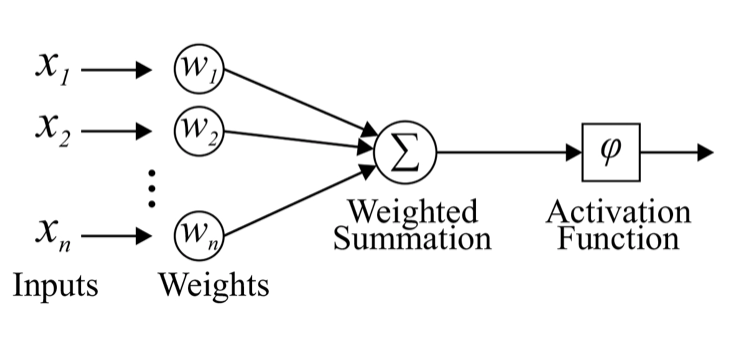
\includegraphics[width=0.6\textwidth]{figures/nn}
            \caption{Perceptron preview. \cite{Mourgias-Alexandris:19}}
            \label{fig:perceptron}
        \end{figure}
    \end{center}
    Neural networks are trained on large datasets using a~process called backpropagation, which adjusts the~weights and biases of the~neurons to minimize the~error between the~predicted output and the~actual output. Once a~neural network has been trained, it can be used to make predictions on new data.\\
    \\
    A neuron is a~basic building block of a~neural network, also known as~an~artificial neuron or a~perceptron.
It is modeled after the~biological neuron in the~human brain, which receives input signals from other neurons,
processes them, and sends output signals to other neurons.\\
    \\
    In a~neural network, a~neuron receives input from other neurons or directly from the~input data, applies a~mathematical function to the~input, and produces~an~output that is sent to other neurons in the~network. The~input to a~neuron is usually a~vector of numbers, and each input is multiplied by a~corresponding weight. The~neuron then sums up the weighted inputs, adds a~bias term, and applies~an~activation function to the~result.\\
    \\
    The purpose of the~activation function is to introduce nonlinearity into the~neuron, which allows the~neural network to learn complex patterns and relationships in the~data. There are several different types of activation functions that can be used, such as the~sigmoid function, ReLU (Rectified Linear Unit) function, and tanh (hyperbolic tangent) function.\\
    \\
    The output of a~neuron is typically fed into other neurons in the~next layer of the~neural network. The~weights and biases of the~neurons are adjusted during the~training process using a~technique called backpropagation, which involves computing the~gradient of the~error with respect to the~weights and updating them using~an~optimization algorithm such as stochastic gradient descent.\\
    \\
    \textbf{Feedforward Neural Networks}\\
    These are the~most basic type of neural networks, where the~information flows only in one direction,from input to output. These networks can have one or more hidden layers and are often used for classification or regression tasks. Shema on basic feedforward NN is on fig~\ref{fig:ff}
    \begin{center}
        \begin{figure}[!ht]
            \centering
            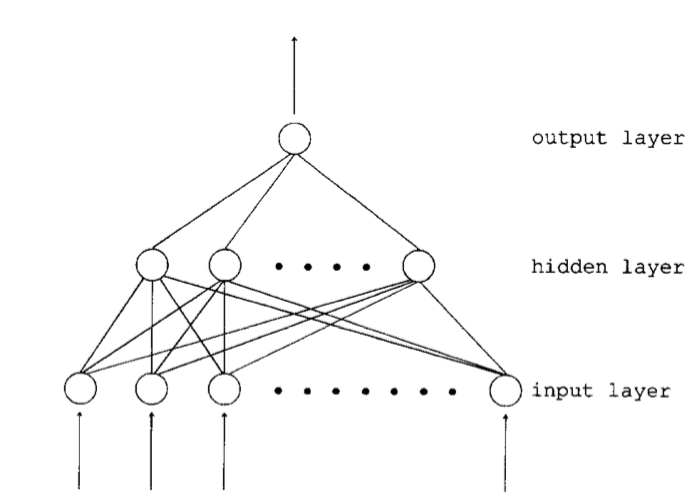
\includegraphics[width=0.6\textwidth]{figures/ff}
            \caption{Typical feed-forward neural network composed of three layers. \cite{svozil1997quantum}}
            \label{fig:ff}
        \end{figure}
    \end{center}
    \textbf{Convolutional Neural Networks (CNNs)}\\
    These networks are specialized for processing images and are commonly used in computer vision tasks. They use convolutional layers to extract features from images and can learn to recognize patterns and objects in images see in fig~\ref{fig:cn}
    \begin{center}
        \begin{figure}[!ht]
            \centering
            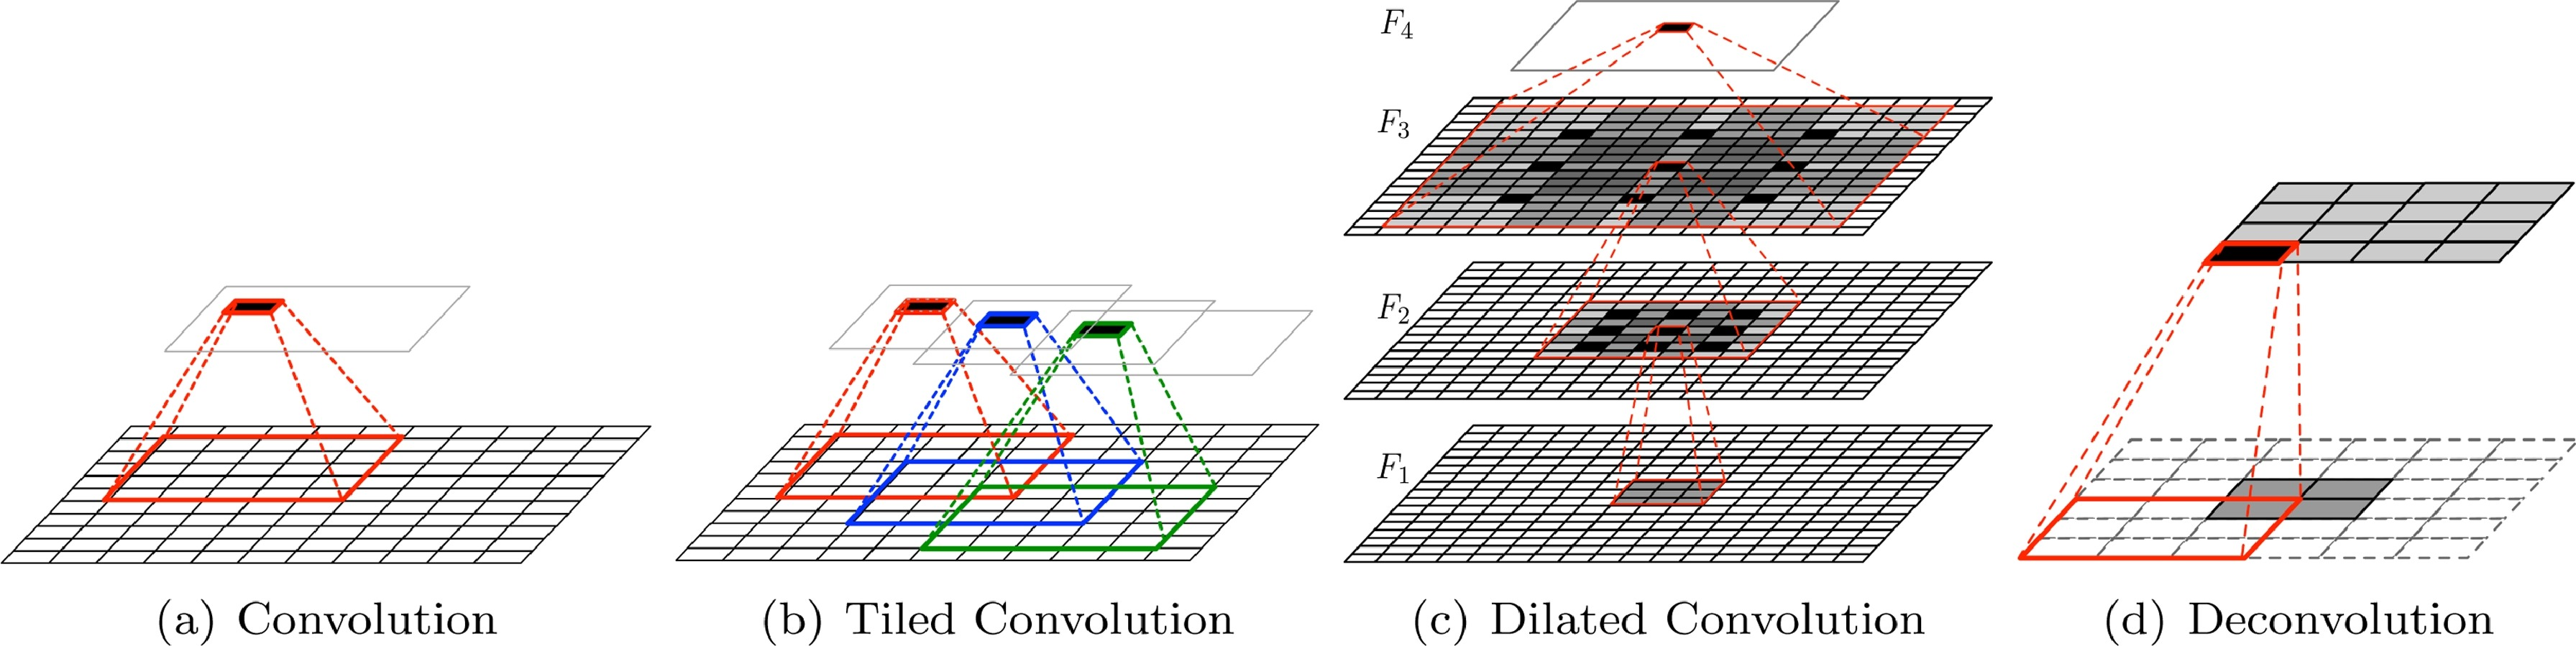
\includegraphics[width=0.8\textwidth]{figures/cn}
            \caption{Illustration of (a) Convolution, (b) Tiled Convolution, (c) Dilated Convolution, and (d)
                Deconvolution. \cite{GU2018354}}
            \label{fig:cn}
        \end{figure}
    \end{center}
    \textbf{Recurrent Neural Networks (RNNs)}\\
    These networks are designed to work with sequential data, such as time-series or natural language data. They have loops that allow information to be passed from one time-step to the~next, enabling them to capture temporal dependencies in the~data, described on fig~\ref{fig:rn}
    \begin{center}
        \begin{figure}[!ht]
            \centering
            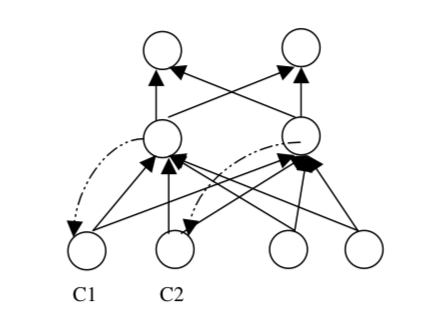
\includegraphics[width=0.4\textwidth]{figures/rn}
            \caption{Typical recurrent network. \cite{medsker2001recurrent}}
            \label{fig:rn}
        \end{figure}
    \end{center}
    \textbf{Long Short-Term Memory Networks (LSTMs)}\\
    These are a~type of RNN that are designed to address the~problem of vanishing gradients in traditional RNNs. They use memory cells and gates to selectively retain or forget information over time, making them well-suited for learning from long sequences. As you can see on fig~\ref{fig:ltmn} color indicates degree of memory activation.
    \begin{center}
        \begin{figure}[!ht]
            \centering
            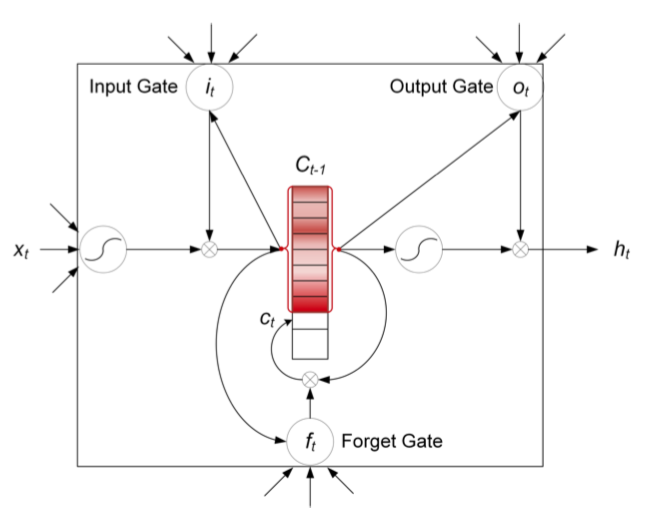
\includegraphics[width=0.35\textwidth]{figures/ltmn}
            \caption{Long short-term memory network. \cite{cheng2016long}}
            \label{fig:ltmn}
        \end{figure}
    \end{center}
    \textbf{Autoencoder Neural Networks}\\
    These networks are used for unsupervised learning and are designed to learn a~compressed representation of the~input data. As we can see on figure~\ref{fig:ann} they consist of~an~encoder that maps the~input data to a~compressed representation, and a~decoder that maps the~compressed representation back to the~original data.
    \begin{center}
        \begin{figure}[!ht]
            \centering
            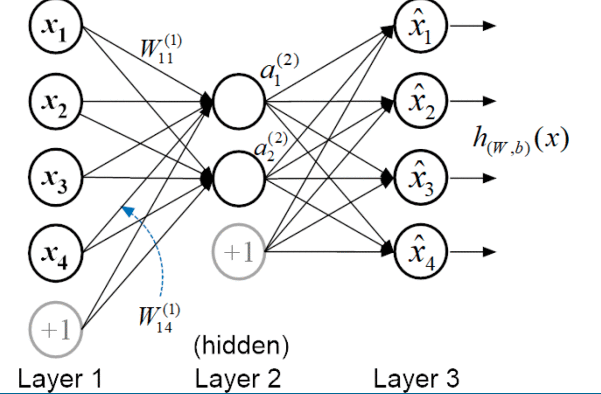
\includegraphics[width=0.5\textwidth]{figures/ann}
            \caption{An autoencoder neural network. \cite{luo2018distributed}}
            \label{fig:ann}
        \end{figure}
    \end{center}
    \textbf{Generative Adversarial Networks (GANs)}\\
    These networks consist of two networks, a~generator and a~discriminator (see on figure~\ref{fig:gan}), that are trained together in a~game-theoretic framework. The~generator is trained to generate realistic data samples, while the~discriminator is trained to distinguish between real and generated data samples.
    \begin{center}
        \begin{figure}[!ht]
            \centering
            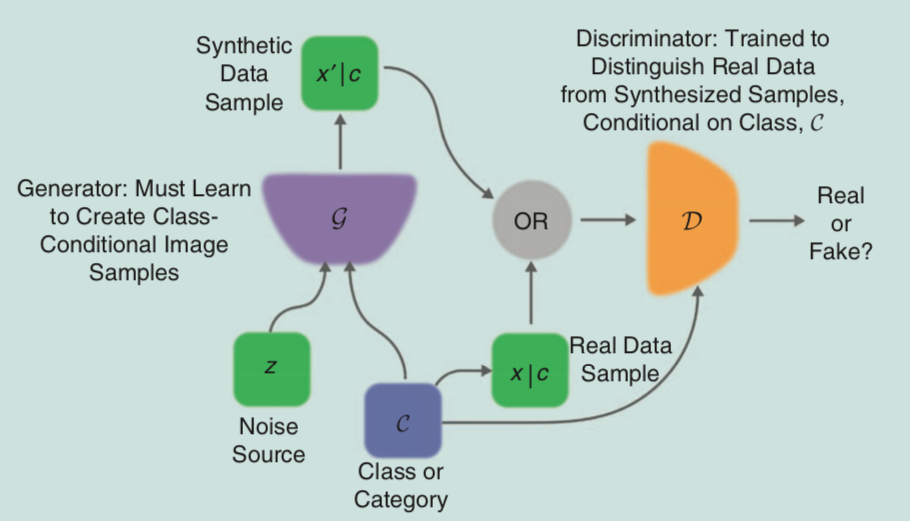
\includegraphics[width=0.5\textwidth]{figures/gan}
            \caption{The conditional GAN schema. \cite{creswell2018generative}}
            \label{fig:gan}
        \end{figure}
    \end{center}
    
    \subsection{Classification} \label{subsec:clasification}
    Neural network data classification is a~technique for categorizing data into different classes or categories based on patterns and features present in the~data. a~neural network is a~type of machine learning algorithm that is modeled after the~structure and function of the~human brain. It is composed of interconnected nodes or neurons that are organized into layers.\\
    \\
    In a~classification task, the~neural network is trained on a~dataset that is labeled with the~correct
class for each example. During training, the~network learns to recognize patterns and features in the~input data
that are associated with each class. The~process of training involves adjusting the~weights and biases of the~neurons in the~network to minimize the~error between the~predicted class and the~actual class of each example in the training set.\\
    \\
    Neural network data classification has been successfully applied to a~wide range of tasks, including image
classification, speech recognition, natural language processing, and fraud detection, among others~\cite{feraud2002methodology}.

    \subsection{Activation functions} \label{subsec:nnaf}
    There are several types of activation functions~\cite{geron2022hands} used in neural networks, as we can see on figure~\ref{fig:activationfunctions} including:
    \begin{itemize}
        \item Sigmoid Function: the~sigmoid function is a~commonly used activation function that maps any input value to a~value between 0 and 1. It is typically used in binary classification problems and in the~output layer of neural networks that produce probability estimates~\ref{fig:sigmoid}.
        \item ReLU (Rectified Linear Unit): the~ReLU function is another popular activation function that maps any input value less than 0 to 0, and any input value greater than or equal to 0 to the~input value itself. It is computationally efficient and has been shown to work well in deep neural networks~\ref{fig:relu}.
        \item Tanh Function: the~tanh (hyperbolic tangent) function is similar to the~sigmoid function, but it maps input values to a~range between -1 and 1. It is commonly used in the~hidden layers of neural networks~\ref{fig:tahn}.
        \item Softmax Function: the~softmax function is often used in the~output layer of neural networks that produce multi-class classification predictions. It maps the~outputs to a~probability distribution over the~possible classes~\ref{fig:sigmsoftmaxoid}.
        \item Leaky ReLU: the~Leaky ReLU function is similar to the~ReLU function, but it allows a~small, non-zero gradient when the~input value is negative. This can help to prevent the~"dying ReLU" problem, where some ReLU units become inactive and stop contributing to the~network's output~\ref{fig:leakyrelu}.
        \item ELU (Exponential Linear Unit): the~ELU function is similar to the~ReLU function, but it allows negative values to have non-zero outputs. This can help to prevent the~"dying ReLU" problem and can improve the performance of deep neural networks~\ref{fig:elu}.
    \end{itemize}
    
    \begin{figure}[!ht]
        \centering
        \begin{subfigure}[b]{0.3\textwidth}
            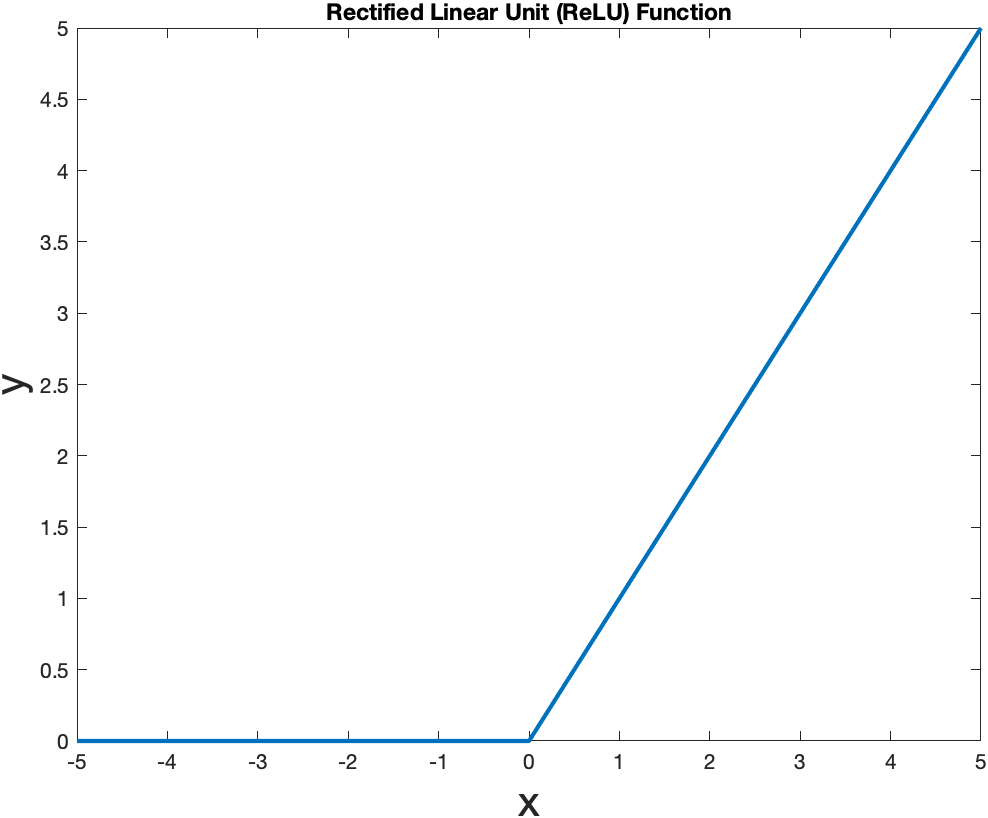
\includegraphics[width=\textwidth]{figures/relu}
            \caption{ReLU}
            \label{fig:relu}
        \end{subfigure}
        \hspace{0.1\textwidth}
        \begin{subfigure}[b]{0.3\textwidth}
            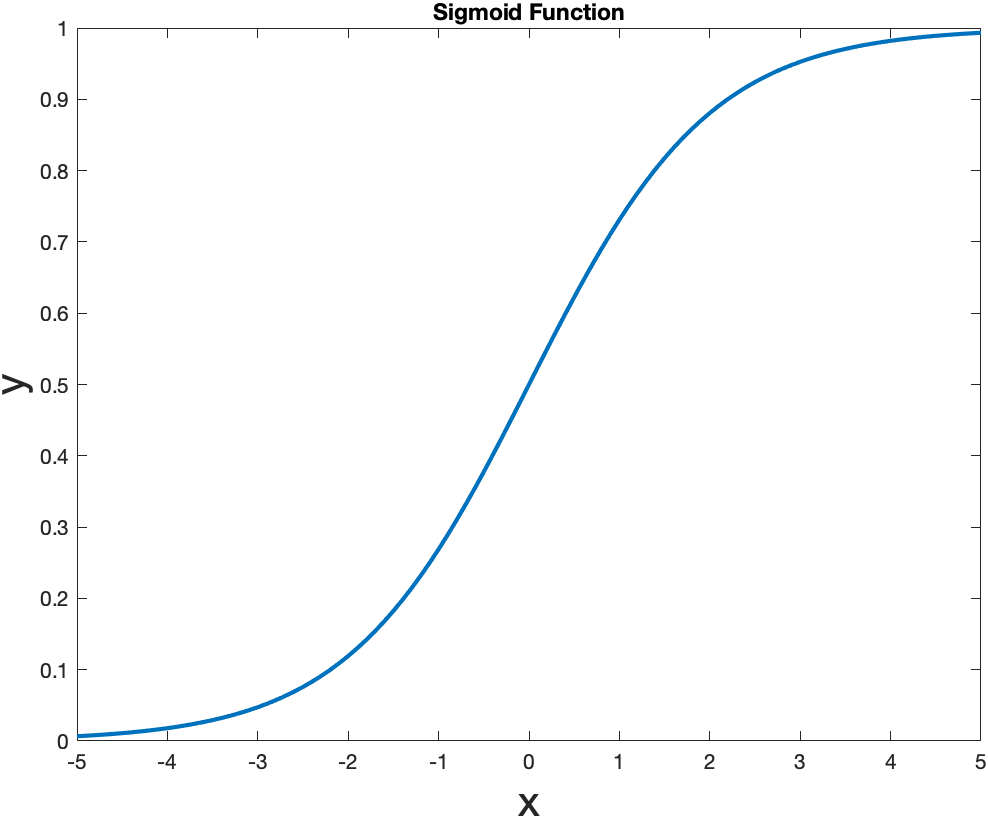
\includegraphics[width=\textwidth]{figures/sigmoid}
            \caption{Sigmoid}
            \label{fig:sigmoid}
        \end{subfigure}
        \begin{subfigure}[b]{0.3\textwidth}
            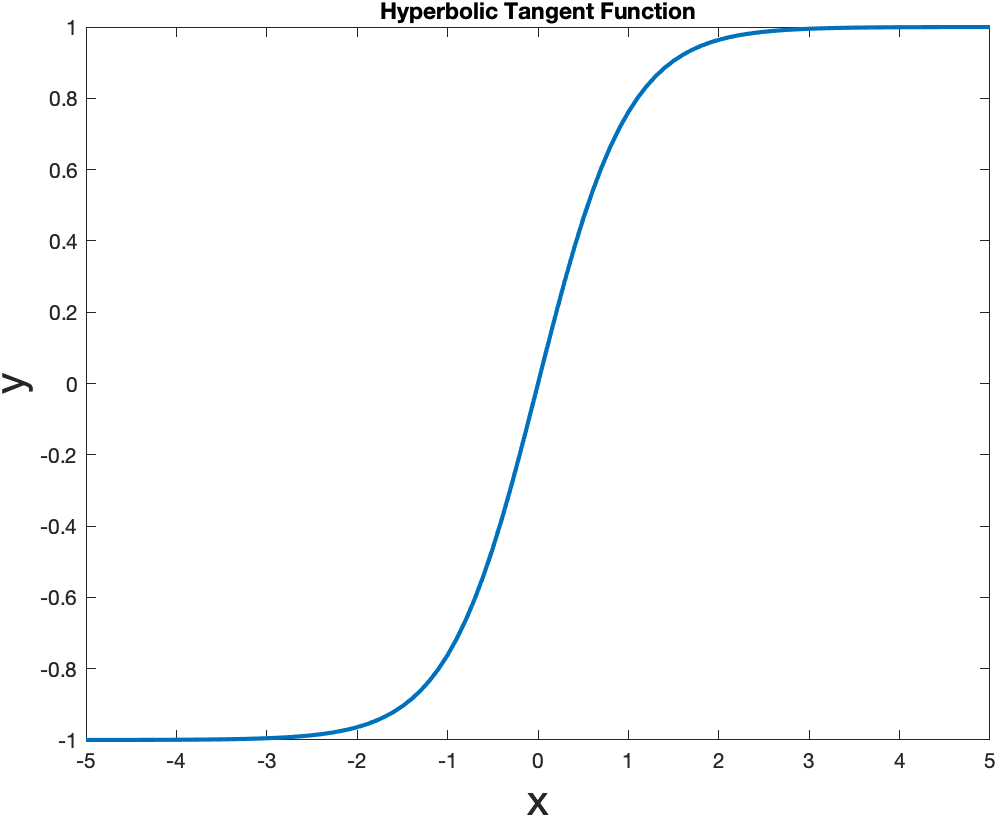
\includegraphics[width=\textwidth]{figures/tanh}
            \caption{Tanh}
            \label{fig:tahn}
        \end{subfigure}
        \hspace{0.1\textwidth}
        \begin{subfigure}[b]{0.3\textwidth}
            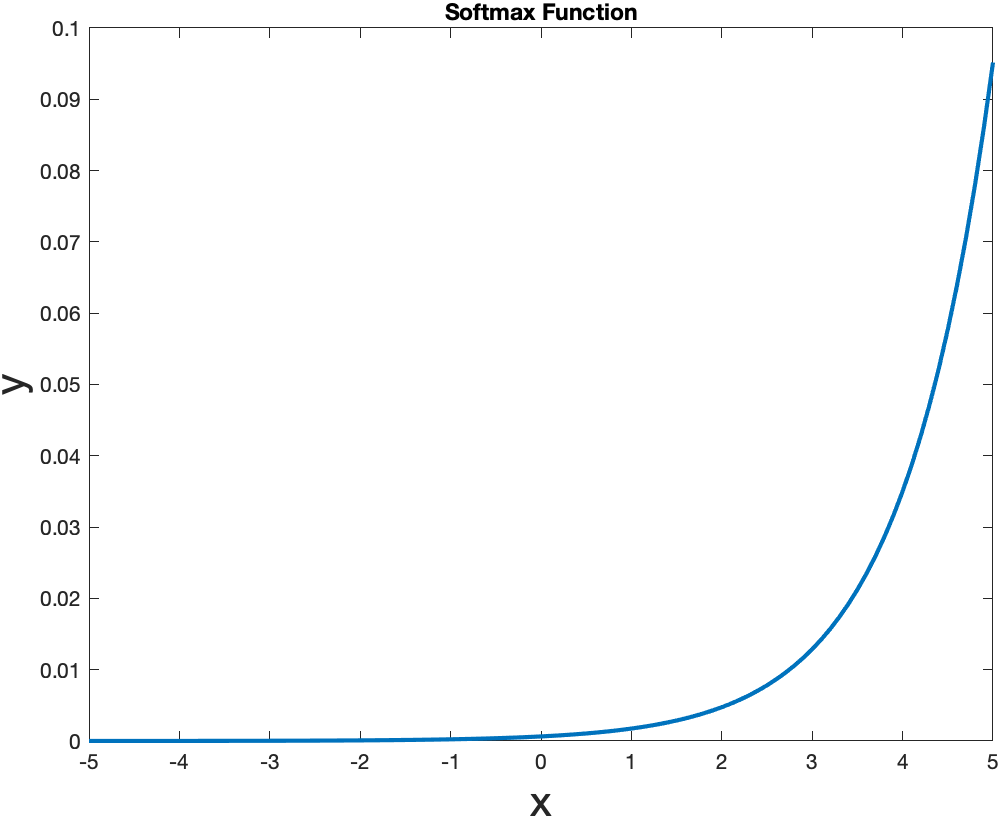
\includegraphics[width=\textwidth]{figures/softmax}
            \caption{Softmax}
            \label{fig:sigmsoftmaxoid}
        \end{subfigure}
        \begin{subfigure}[b]{0.3\textwidth}
            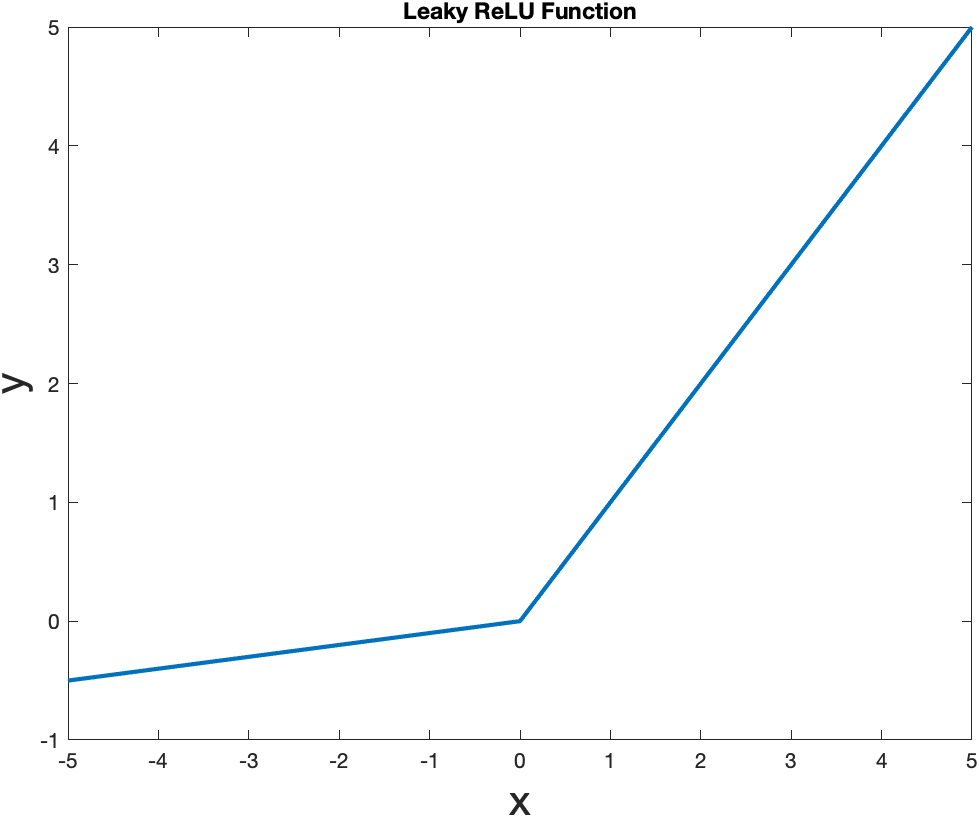
\includegraphics[width=\textwidth]{figures/leakyrelu}
            \caption{Leaky ReLU}
            \label{fig:leakyrelu}
        \end{subfigure}
        \hspace{0.1\textwidth}
        \begin{subfigure}[b]{0.3\textwidth}
            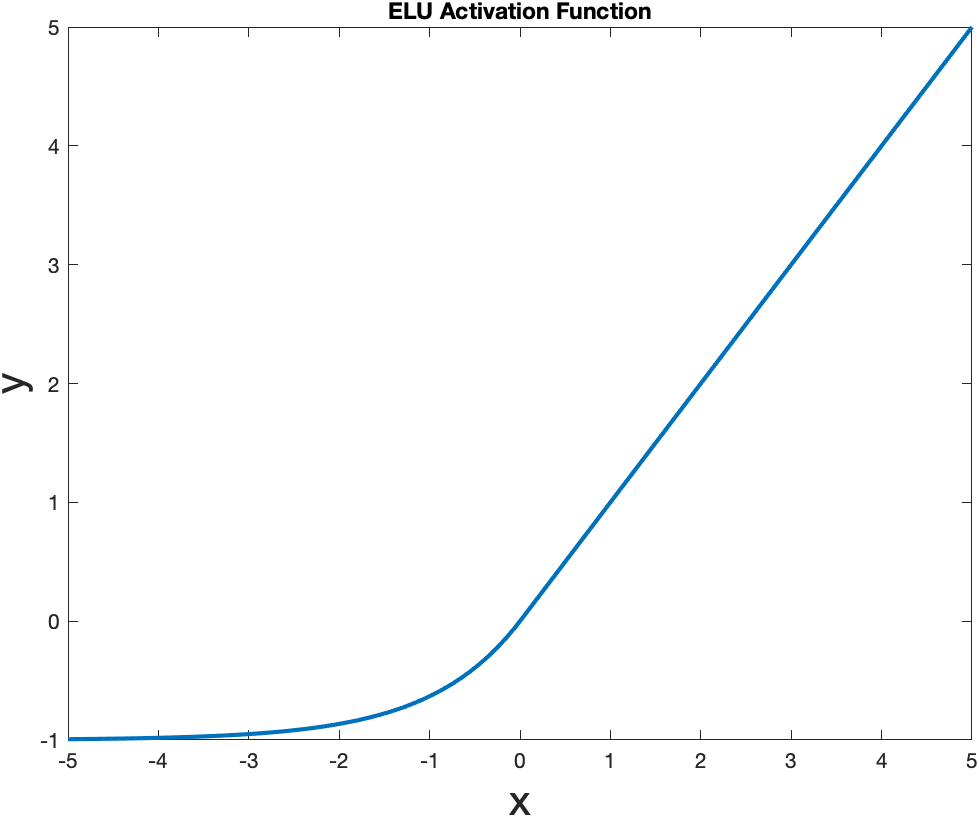
\includegraphics[width=\textwidth]{figures/elu}
            \caption{ELU}
            \label{fig:elu}
        \end{subfigure}
        \caption{Neural network activation functions.}
        \label{fig:activationfunctions}
    \end{figure}

    \noindent These are some of the~most commonly used activation functions in neural networks,
    but there are many other types of activation functions that have been developed
    for specific tasks or to address certain problems.
\chapter{Implementation}
    The proposed project is focused on the design and development of the \emph{Automatic prediction model builder system} in the form of an application with an user-friendly interface, implemented in the cloud environment, and that uses all the principles described in~\ref{analysis}. As the development environment Matlab ecosystem was used.

    \section{Mathematical models}
    The implemented prediction models are based mainly on the principle of linear prediction (LP) and its modifications, such as non-integer linear prediction (fractional-order linear prediction - FLP), LP extended by parameters capable of capturing short-term and long-term trendiness in data (extended linear prediction - ELP), etc., that were developed by the author and his supervisor. These approaches are extended by further statistical methods such as Monte Carlo, Markov chains, etc.
    
        For the identification of the appropriate structure of economic and behavioural models and the identification of the parameters of the selected models, machine learning algorithms are used, which provide the optimal solution for the selected data and thus the use-case.
 
    \section{Application}
    The developed application makes it possible to easily and accurately predict various socioeconomic macro and micro indicators, such as gross/net domestic/national product, economic wealth, unemployment, inflation, average/minimum wage, purchasing power of the population but also the behaviour of customers (customers can also be perceived as households), intended for sectors such as public or state administration, public planning (but also private) finance, banking.
    
    From the point of view of commercial use, a possible application would be predicting the number of customers and the number of orders, the company's income, the success of marketing strategies, or based on the prediction, the planning of the warehouse stocks.

%    \begin{figure}
%        \centering
%        \begin{subfigure}[b]{0.4\textwidth}
%            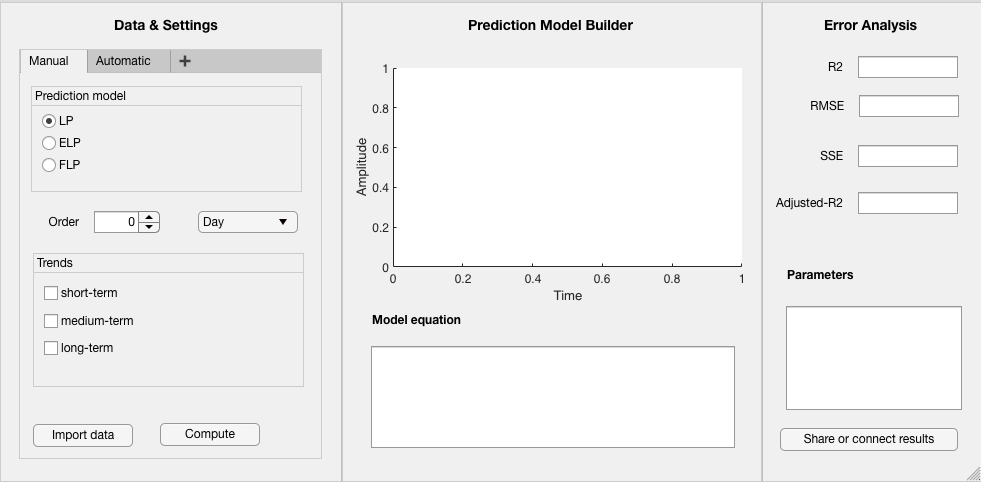
\includegraphics[width=\textwidth]{figures/manual.png}
%            \caption{Manual settings}
%            \label{fig:manual}
%        \end{subfigure}
%        \hspace{0.1\textwidth}
%        \begin{subfigure}[b]{0.4\textwidth}
%            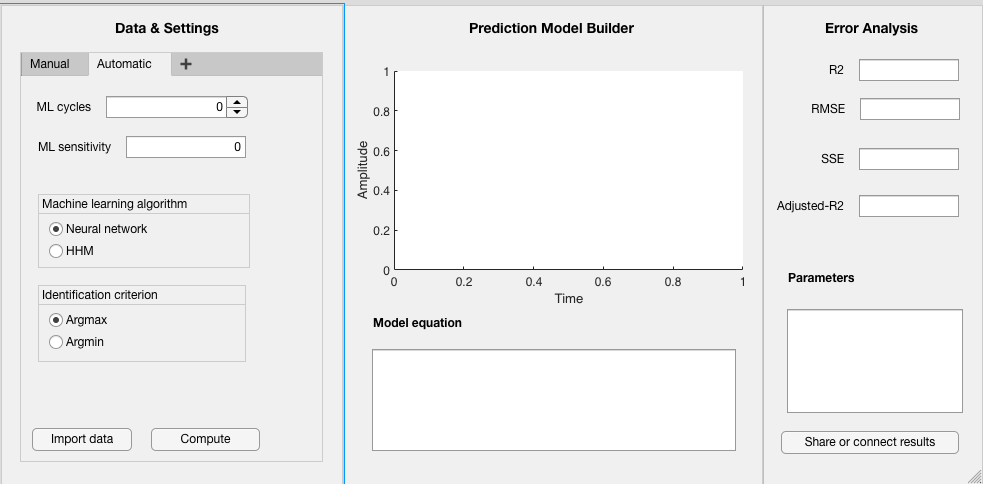
\includegraphics[width=\textwidth]{figures/auto.png}
%            \caption{Automatic settings}
%            \label{fig:automatic}
%        \end{subfigure}
%        \begin{subfigure}[b]{0.4\textwidth}
%            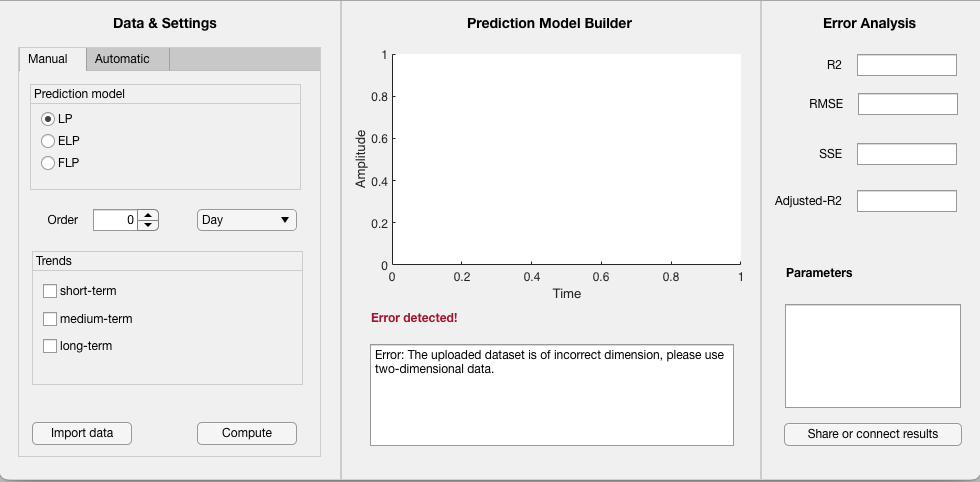
\includegraphics[width=\textwidth]{figures/warning.png}
%            \caption{Dataset warning}
%            \label{fig:warning}
%        \end{subfigure}
%        \hspace{0.1\textwidth}
%        \begin{subfigure}[b]{0.4\textwidth}
%            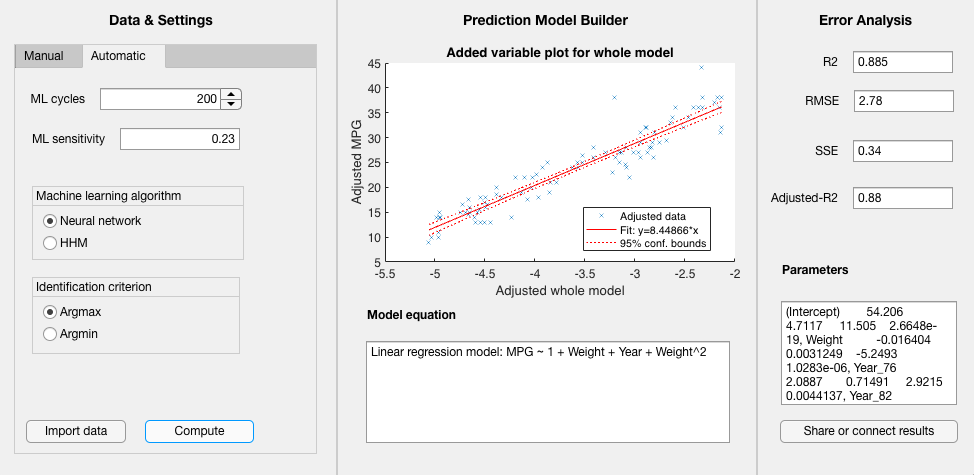
\includegraphics[width=\textwidth]{figures/result.png}
%            \caption{Results}
%            \label{fig:results}
%        \end{subfigure}
%        \label{fig:appoverview}
%        \caption{Application overview}
%    \end{figure}


        \subsection{Dataset import}
 
       To import the dataset to be processed, one has to use the button in the left
        bottom corner~(Fig.~\ref{fig:manual}). Application is able to
        process datasets in *.csv or *.xlsx format. The dataset is firstly checked, if it is of correct format, and in the case of error a warning is shown (Fig.~\ref{fig:warning}) with the tips
        how to format the uploaded dataset.
               \begin{figure}[h!]
        \centering
            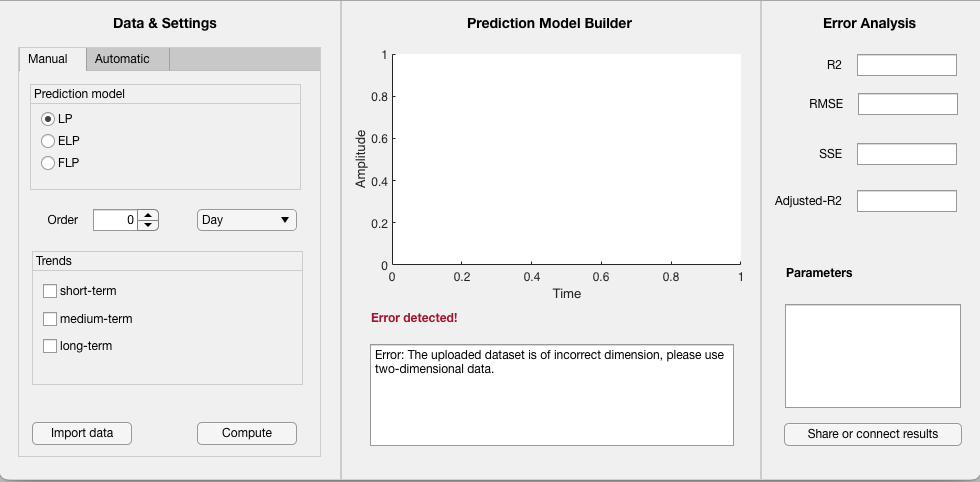
\includegraphics[width=\textwidth]{figures/warning.png}
            \caption{Dataset warning}
            \label{fig:warning}
    \end{figure}

        
        \subsection{Settings}\label{subsec:setting}
        The developed application has two main possibilities of settings, one can decide to choose a mathematical model and set other related parameters manually (Fig.~\ref{fig:manual}), or to choose automatic settings (Fig.~\ref{fig:automatic}) of application to detect the best prediction model
        based on uploaded dataset.\\
        \\
        \textbf{Manual settings}\\
     In the \emph{Manual settings} environment one is allowed to choose a prediction model (one among three) based on the type of linear prediction and to set two other settings:
  %
       \begin{figure}[h!]
        \centering
	   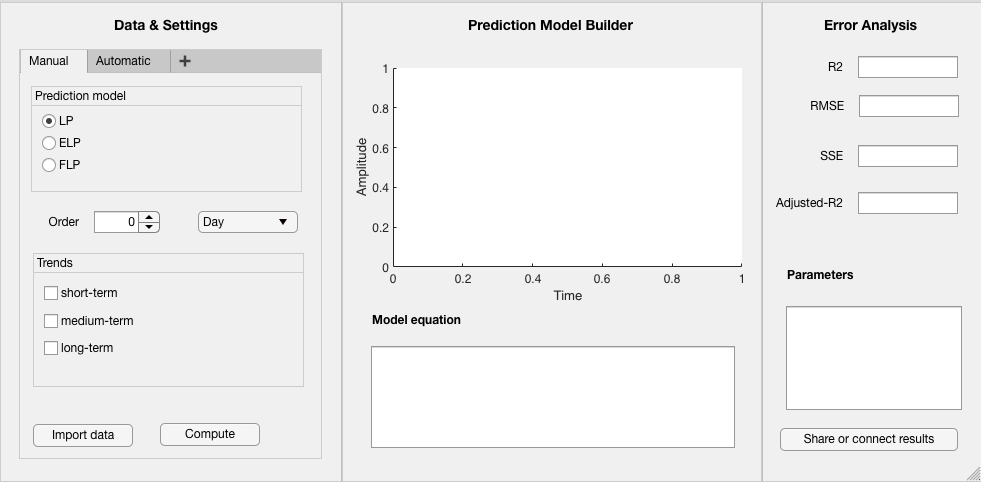
\includegraphics[width=\textwidth]{figures/manual.png}
            \caption{Manual settings}
            \label{fig:manual}
    \end{figure}



        \begin{itemize}
            \item \textbf{Prediction models}\\
            One can choose one of three types of linear prediction, \emph{Standard linear prediction}~\ref{eg:lp}, \emph{Extended linear prediction}~\ref{eg:elp},
            and \emph{Fractional-order linear prediction}~\ref{eg:flp}.\\
      \\
     The Standard linear prediction can be defined as:
     % 
                 \begin{equation}\label{eg:lp}
                \hat{x}(n) = \sum_{i=1}^{p} a_i x(n-i),
                \label{eq:linear-predictor}
            \end{equation}
              %
            where $\hat{x}(n)$ is the~predicted value of $x(n)$, $p$ is the~order of the~predictor, and $a_i$ are the~predictor coefficients. The~predictor coefficients can be found by minimizing the~prediction error.
                        \\
                        \\
    The Extended linear prediction can be defined as:
%
                 \begin{equation}\label{eg:elp}
                \hat{x}(n) = \left(\sum_{i=1}^{p} a_i x(n-i) + \sum_{i=1}^{q} b_i x(n-S-i)\right) \gamma(n),
            \end{equation}
           %
            where $\hat{x}(n)$ is the~predicted value of the~order at time $n$, $x(n-i)$ is the~past short-therm prediction part $p$ samples of the~dataset, $x(n-S-i)$ is the~past long-term prediction part with seasonal shift $S$, and $a_i$ and $b_i$ are the~predictors coefficients. The~order of the~predictor is $p$ for short-term and $q$ for the long-term linear prediction. The seasonal weights are represented by $\gamma(n)$.\\
                                    \\
    The Fractional-order linear prediction can be defined as:
            \\
            \begin{equation}\label{eg:flp}
                \hat{x}(n) = \frac{a}{h^\alpha}(x(n-1) - \alpha x(n-2)),
                \label{eq:linear-predictor}
            \end{equation}
            %
            that uses two-samples memory, is dependent on one parameter $a$ and the order of fractional derivative $\alpha$~\cite{skovranek}
.
           
            \item \textbf{Prediction order}\\
            In this step we are able to set up the order of linear prediction and the
            period of predicted values.
            \item \textbf{Trends detection}\\
            In this setting you are able to choose the length of the period to 
            identify the prediction model parameters and trends.
        \end{itemize}
        \noindent
        \\
        \textbf{Automatic settings}\\
        The \emph{Automatic settings} can be used to set up the parameters of neural network,
        which is used to estimate optimal parameters for prediction. 
                  %
       \begin{figure}[h!]
        \centering
            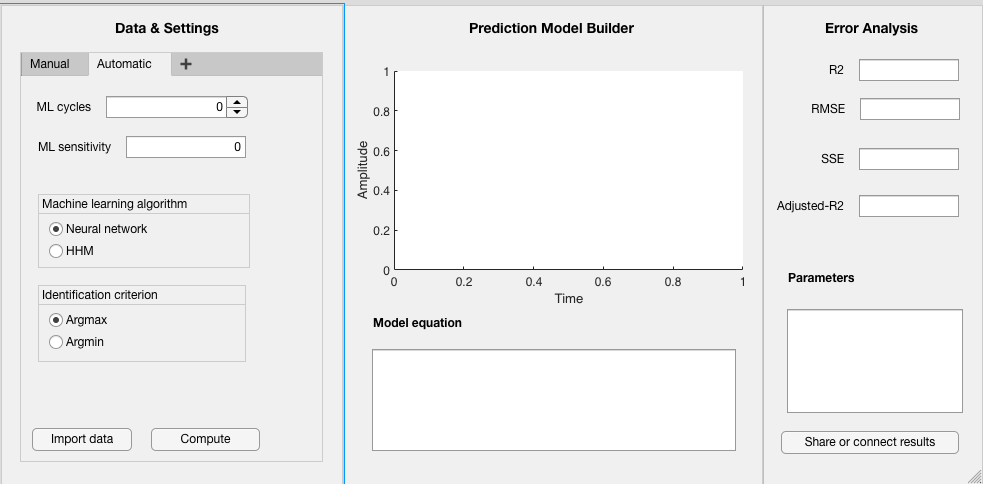
\includegraphics[width=\textwidth]{figures/auto.png}
            \caption{Automatic settings}
            \label{fig:automatic}
    \end{figure}
        %
                For the set up of automation part of application we are able to use these parameters:\\
        \begin{itemize}
            \item \textbf{Machine learning cycles}\\
            Number of observations used to find optimal parameters of the model.
            \item \textbf{Machine learning sensitivity}\\
            Sensitivity is a measure of how well a machine learning model can
            detect positive instances. It is also known as the true positive rate
            (TPR) or recall.
            \item \textbf{Machine learning algorithms}\\
            In this section we are able to choose the neural network or hidden Markov model
            to run in background. HMM is statistical approach and in specific dataset can provide
            better results.
            \item \textbf{Identification criteria}\\
            In this part we can choose the maximisation or minimisation as the criterion
            to find optimal parameters.
        \end{itemize}
   
        \subsection{Results}\label{subsec:result}
        For the test purpose, we used the automatic settings of the application and run the application with the uploaded
       dataset. Figure~\ref{fig:results} shows the results of the developed application.
       %
               \begin{figure}[h!]
        \centering
            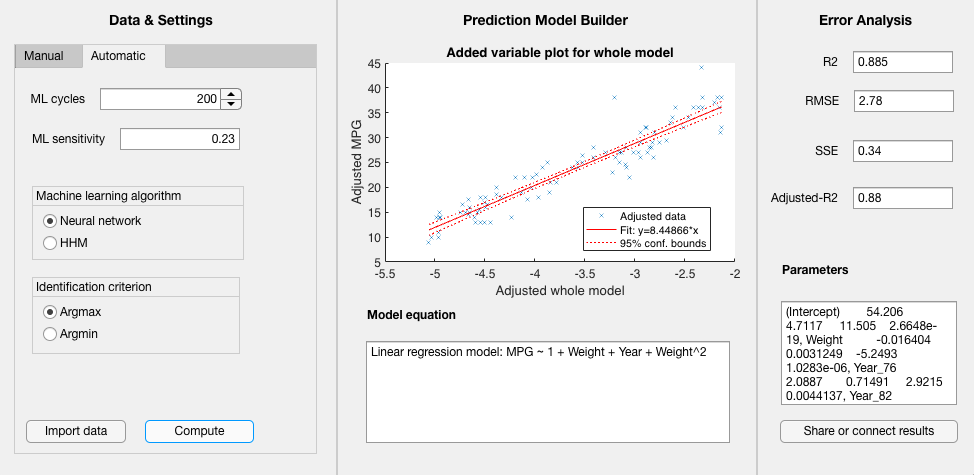
\includegraphics[width=\textwidth]{figures/result.png}
            \caption{Results}
            \label{fig:results}
    \end{figure}
        %
        Application successfully detects the model equation, identifies optimal parameters and 
        calculates the fitting criteria. Model builder creates the model with $R^2 = 0.885$.
        The application displays the results in these four sections:\\
        \\
        \textbf{Plot of results}\\
       Figure~\ref{fig:results} shows the main window of the application, where in the middle of the screen
       the uploaded dataset as well as the moddeled fitting-curve are plotted.\\
        \\
        \textbf{Model equation}\\
        Under the main section with plotted results, one can find the model equation section, where
       the mathematical model proposed by the application is shown.\\
        \\
        \textbf{Parameters}\\
        In the right bottom corner one can see the parameters of the identified model. When the
        Model equation and Parameters section are combined, we are able to use the created model in other
        applications and approaches if necessary.\\
        \\
        \textbf{Error Analysis}\\
        The last part of the application is Error Analysis, where we can find the 
        results of the created model. Application provides $R^2$, adjusted $R^2$,
        Root Mean Square Error and Sum Squared Error.
        
        

% good linebraking of bibtex url
\setcounter{biburllcpenalty}{7000}
\setcounter{biburlucpenalty}{8000}

%% The bibliography
\printbibliography[heading=bibintoc]

\label{theend} % the last page of the thesis


\end{document}